\documentclass[11pt,a4paper]{article}

% Image mode: pdf.
% Image paths stay relative. In PDF mode, place same-basename PDF conversions
% of the chapter SVG files in the assets/ directory beside this source.

\usepackage{iftex}
\ifPDFTeX
  \PackageError{handout}{This template requires XeTeX or Tectonic}{Compile with xelatex or tectonic.}
\fi

\usepackage[a4paper,top=18mm,bottom=20mm,left=20mm,right=20mm,headsep=6mm]{geometry}
\usepackage{fontspec}
\usepackage{xeCJK}
\usepackage{amsmath}
\usepackage{unicode-math}

% Font settings are intentionally visible in the generated .tex file.
% These defaults target the macOS machine used for the released PDF.
% Change the family names when compiling on another system.
\setmainfont{Songti TC}
\setsansfont{Heiti TC}
\setmonofont{Menlo}
\setCJKmainfont{Songti TC}
\setCJKsansfont{Heiti TC}
\setCJKmonofont{Heiti TC}
\setmathfont{STIX Two Math}
\XeTeXlinebreaklocale "zh"
\XeTeXlinebreakskip=0pt plus 1pt

\usepackage{xcolor}
\definecolor{HandoutBlue}{HTML}{215A91}
\definecolor{HandoutBlueLight}{HTML}{EEF5FC}
\definecolor{HandoutGreen}{HTML}{39715A}
\definecolor{HandoutGreenLight}{HTML}{EFF8F3}
\definecolor{HandoutGold}{HTML}{8A641C}
\definecolor{HandoutGoldLight}{HTML}{FFF8E8}
\definecolor{HandoutInk}{HTML}{253142}
\definecolor{HandoutMuted}{HTML}{667085}

\usepackage{graphicx}
\makeatletter
% Pandoc 3 emits an accessibility `alt` key for raster/PDF images. Older
% graphicx releases do not know that key, so accept it without changing layout.
\@ifundefined{KV@Gin@alt}{\define@key{Gin}{alt}{}}{}
\newsavebox\pandoc@box
\newcommand*\pandocbounded[1]{%
  \sbox\pandoc@box{#1}%
  \Gscale@div\@tempa{\textheight}{\dimexpr\ht\pandoc@box+\dp\pandoc@box\relax}%
  \Gscale@div\@tempb{\linewidth}{\wd\pandoc@box}%
  \ifdim\@tempb\p@<\@tempa\p@\let\@tempa\@tempb\fi
  \ifdim\@tempa\p@<\p@\scalebox{\@tempa}{\usebox\pandoc@box}%
  \else\usebox{\pandoc@box}%
  \fi
}
\makeatother
\usepackage{float}
\floatplacement{figure}{H}
% Pandoc uses LTcaptype=none for uncaptioned longtables. The caption package
% expects that name to exist as a counter even though it is never displayed.
\newcounter{none}
\usepackage{caption}
\captionsetup[figure]{labelformat=empty,labelsep=none,font=small}

\usepackage{booktabs,longtable,array,calc}
\usepackage{etoolbox}
\makeatletter
\patchcmd\longtable{\par}{\if@noskipsec\mbox{}\fi\par}{}{}
\makeatother

\usepackage[most]{tcolorbox}
\tcbuselibrary{breakable,skins}
\newtcolorbox{HandoutLearningMap}{
  enhanced,breakable,colback=HandoutBlueLight,colframe=HandoutBlue,
  boxrule=0.8pt,arc=1.5mm,left=3mm,right=3mm,top=2mm,bottom=2mm,
  before skip=8pt,after skip=10pt
}
\newtcolorbox{HandoutWorkedExample}{
  enhanced,breakable,colback=HandoutGreenLight,colframe=HandoutGreen,
  boxrule=0.65pt,arc=1.5mm,left=3mm,right=3mm,top=2mm,bottom=2mm,
  before skip=8pt,after skip=10pt
}
\newtcolorbox{HandoutSelfCheck}{
  enhanced,breakable,colback=HandoutGoldLight,colframe=HandoutGold,
  boxrule=0.65pt,arc=1.5mm,left=3mm,right=3mm,top=2mm,bottom=2mm,
  before skip=8pt,after skip=10pt
}

\usepackage{titlesec}
\titleformat{\section}{\sffamily\bfseries\Large\color{HandoutBlue}}{}{0pt}{}
\titleformat{\subsection}{\sffamily\bfseries\large\color{HandoutInk}}{}{0pt}{}
\titleformat{\subsubsection}{\sffamily\bfseries\normalsize\color{HandoutInk}}{}{0pt}{}
\titlespacing*{\section}{0pt}{1.4em}{0.55em}
\titlespacing*{\subsection}{0pt}{1.15em}{0.45em}
\titlespacing*{\subsubsection}{0pt}{0.9em}{0.35em}
\setcounter{secnumdepth}{-\maxdimen}

\usepackage{hyperref}
\usepackage{bookmark}
\IfFileExists{xurl.sty}{\usepackage{xurl}}{}
\urlstyle{same}
\hypersetup{
  colorlinks=true,
  linkcolor=HandoutBlue,
  urlcolor=HandoutBlue,
  citecolor=HandoutBlue,
  pdftitle={數2-1 數列與級數},
  pdfsubject={數學},
  pdfcreator={Pandoc with the HighSchooContent LaTeX template}
}

\setlength{\parindent}{0pt}
\setlength{\parskip}{0.55em plus 0.15em minus 0.1em}
\setlength{\emergencystretch}{3em}
\setlength{\LTpre}{0.5em}
\setlength{\LTpost}{0.5em}
\renewcommand{\arraystretch}{1.18}
\providecommand{\tightlist}{%
  \setlength{\itemsep}{0pt}\setlength{\parskip}{0pt}}
\pagestyle{plain}


\begin{document}

\begin{tcolorbox}[
  enhanced,colback=white,colframe=HandoutBlue,boxrule=1.1pt,arc=2mm,
  borderline west={3pt}{0pt}{HandoutBlue},left=5mm,right=4mm,top=4mm,bottom=4mm
]
{\sffamily\small\bfseries\color{HandoutBlue}學生講義}\par
{\sffamily\bfseries\LARGE\color{HandoutInk}數2-1 數列與級數}\par
\vspace{0.35em}{\large 用索引、遞迴與部分和描述逐期變化及累積結果}\par
\vspace{0.45em}{\small\color{HandoutMuted}%
科目：數學
\quad 課程：普通高中數學 第二冊
\quad 版本：學生版｜核心＋理解
\quad 校訂：2026-08-29
}\par
\vspace{0.25em}{\small\color{HandoutMuted}範圍：114 學年度數學第二冊第 1 章；數列、等差與等比、遞迴、數學歸納法、有限級數及財務應用}\par
\end{tcolorbox}


\begin{HandoutLearningMap}

\subsection{本章問題與能力}\label{ux672cux7ae0ux554fux984cux8207ux80fdux529b}

\begin{enumerate}
\def\labelenumi{\arabic{enumi}.}
\tightlist
\item
  如何用第 \(n\) 項 \(a_n\) 描述按順序出現的資料？
\item
  固定增加量與固定倍率，分別形成什麼數列？
\item
  只知道初始值與更新規則時，如何產生並分析整個數列？
\item
  數學歸納法如何證明對每個正整數都成立的命題？
\item
  如何快速計算等差、等比及常用有限級數？
\item
  單利、複利與定期存款的時間結構如何轉成數列與級數？
\end{enumerate}

本章路徑：數列與通項 → 等差與等比 → 遞迴與歸納 → 有限級數 → 常用和式 → 逐期累積模型。

\end{HandoutLearningMap}

\section{0. 本章用途：描述每一期，也計算累積總量}\label{ux672cux7ae0ux7528ux9014ux63cfux8ff0ux6bcfux4e00ux671fux4e5fux8a08ux7b97ux7d2fux7a4dux7e3dux91cf}

許多資料同時帶有「順序」與「數值」。第 1 年到第 10 年的資產、第 1 排到第 20 排的座位數、每次反射後的光強、演算法第 \(n\) 步的操作量，都可依順序記成數列。通項回答指定一期的數值；遞迴式則直接表達「下一期如何由前一期更新」。

級數處理累積量。前 \(n\) 排的總座位、前 \(n\) 期的總投入、分段圖案的總長度，都由 \(a_1+\cdots+a_n\) 計算。等差級數利用首尾配對，等比級數利用錯位相減，把逐項相加轉成可直接計算的公式。

利息模型把這兩種結構放在同一條時間軸上。單利每期增加固定金額，對應等差變化；複利每期乘固定倍率，對應等比變化；固定存款的期末總額，則是不同存入時間所形成的等比級數。模型成立的條件包含固定期利率、明確的存款時點，以及每一期長度一致。

\section{1. 數列、索引與通項}\label{ux6578ux5217ux7d22ux5f15ux8207ux901aux9805}

\subsection{1.1 數列的定義}\label{ux6578ux5217ux7684ux5b9aux7fa9}

按照確定順序排列的一串數稱為\textbf{數列}，依序記作

\[
a_1,a_2,a_3,\ldots
\]

或簡記為 \(\langle a_n\rangle\)。\(a_n\) 是第 \(n\) 項，\(n\) 是正整數索引。只含有限項的是有限數列；項數可持續增加的是無窮數列。本章的級數公式處理前 \(n\) 項，因此每次計算仍是有限累積。

數列可視為定義域為正整數的函數：輸入 \(n\)，輸出 \(a_n\)。只有整數索引上的點屬於此數列；連線用來協助辨認趨勢。

\begin{figure}
\centering
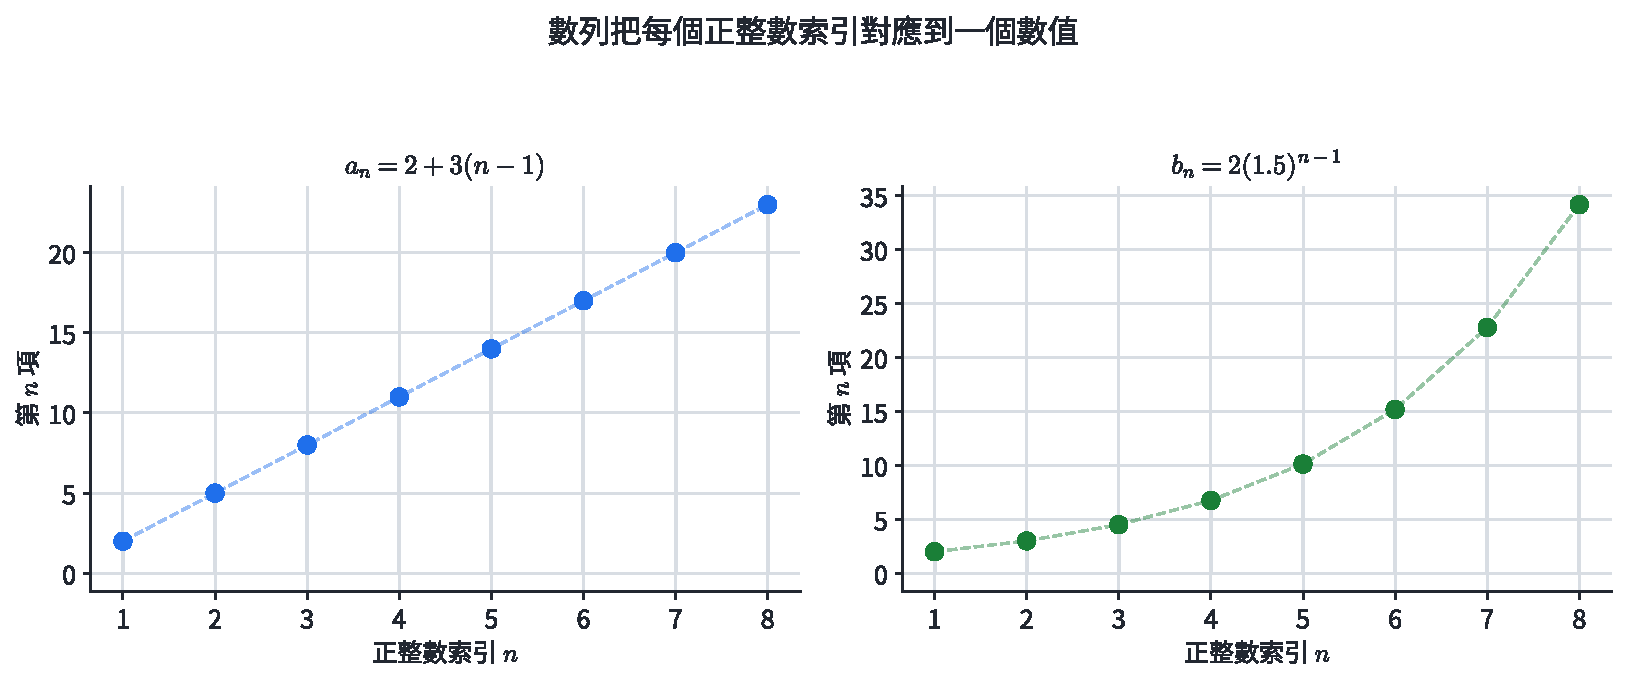
\includegraphics[width=0.94\linewidth,height=\textheight,keepaspectratio,alt={同一組索引可對應等差或等比數值；圖上的點由公式直接計算}]{assets/數2-1-數列是離散對應.pdf}
\caption{同一組索引可對應等差或等比數值；圖上的點由公式直接計算}
\end{figure}

若有一個式子能由 \(n\) 直接算出 \(a_n\)，這個式子稱為數列的\textbf{通項公式}。通項同時處理兩個方向：給定 \(n\) 求項值，或給定項值解出可能的索引。

\subsection{例 1｜由通項讀出符號與大小}\label{ux4f8b-1ux7531ux901aux9805ux8b80ux51faux7b26ux865fux8207ux5927ux5c0f}

已知

\[
a_n=(-1)^{n+1}(2n-1).
\]

求前五項與 \(a_{20}\)。

當 \(n\) 為奇數時，\((-1)^{n+1}=1\)；當 \(n\) 為偶數時，\((-1)^{n+1}=-1\)。逐項代入：

\[
a_1=1,\quad a_2=-3,\quad a_3=5,\quad a_4=-7,\quad a_5=9.
\]

又

\[
a_{20}=(-1)^{21}(39)=-39.
\]

索引控制兩件事：\(2n-1\) 控制絕對值，\((-1)^{n+1}\) 控制正負交替。

\subsection{例 2｜由項值反求索引}\label{ux4f8b-2ux7531ux9805ux503cux53cdux6c42ux7d22ux5f15}

數列的通項為

\[
b_n=\frac{n+1}{2n-1}.
\]

判斷 \(\dfrac6{11}\) 是第幾項。

令 \(b_n=\dfrac6{11}\)：

\[
\frac{n+1}{2n-1}=\frac6{11}
\quad\Longrightarrow\quad
11n+11=12n-6.
\]

所以 \(n=17\)。代回得 \(b_{17}=18/33=6/11\)，且 \(17\) 是正整數，因此它是第 17 項。

\subsection{1.2 分節練習}\label{ux5206ux7bc0ux7df4ux7fd2}

\begin{enumerate}
\def\labelenumi{\arabic{enumi}.}
\tightlist
\item
  已知 \(a_n=n^2-3n\)，寫出前四項並求 \(a_{12}\)。
\item
  已知 \(b_n=3\cdot2^{n-1}\)，求第一個大於 \(1000\) 的項及其索引。
\item
  為數列 \(2,-4,6,-8,\ldots\) 寫出一個通項，並求第 15 項。
\item
  已知 \(c_n=\dfrac{n+1}{2n-1}\)，求滿足 \(c_n=6/11\) 的索引。
\item
  階梯教室第 1 排有 18 個座位，之後每排比前一排多 2 個。先只用索引表示第 \(n\) 排座位數，再求第 15 排。
\end{enumerate}

\subsection{1.3 分節練習解析}\label{ux5206ux7bc0ux7df4ux7fd2ux89e3ux6790}

\begin{enumerate}
\def\labelenumi{\arabic{enumi}.}
\tightlist
\item
  代入 \(n=1,2,3,4\) 得 \(-2,-2,0,4\)；\(a_{12}=12^2-3(12)=108\)。
\item
  依序比較 \(3\cdot2^{n-1}\)。\(b_9=3\cdot2^8=768\)，\(b_{10}=3\cdot2^9=1536\)，故答案是第 10 項 \(1536\)。
\item
  絕對值為 \(2n\)，奇數項為正，因此可取 \(a_n=2n(-1)^{n+1}\)；\(a_{15}=30\)。
\item
  解 \(11(n+1)=6(2n-1)\) 得 \(n=17\)。
\item
  從第 1 排到第 \(n\) 排經過 \(n-1\) 次增加，故 \(a_n=18+2(n-1)=2n+16\)，\(a_{15}=46\) 個。
\end{enumerate}

\section{2. 等差數列與等比數列}\label{ux7b49ux5deeux6578ux5217ux8207ux7b49ux6bd4ux6578ux5217}

\subsection{2.1 等差數列：每一步增加固定量}\label{ux7b49ux5deeux6578ux5217ux6bcfux4e00ux6b65ux589eux52a0ux56faux5b9aux91cf}

若數列從第二項起都滿足

\[
a_n-a_{n-1}=d,\qquad n\ge2,
\]

則稱為\textbf{等差數列}，常數 \(d\) 稱為公差。由 \(a_1\) 走到 \(a_n\) 共經過 \(n-1\) 次加法，因此

\[
\boxed{a_n=a_1+(n-1)d}.
\]

\begin{figure}
\centering
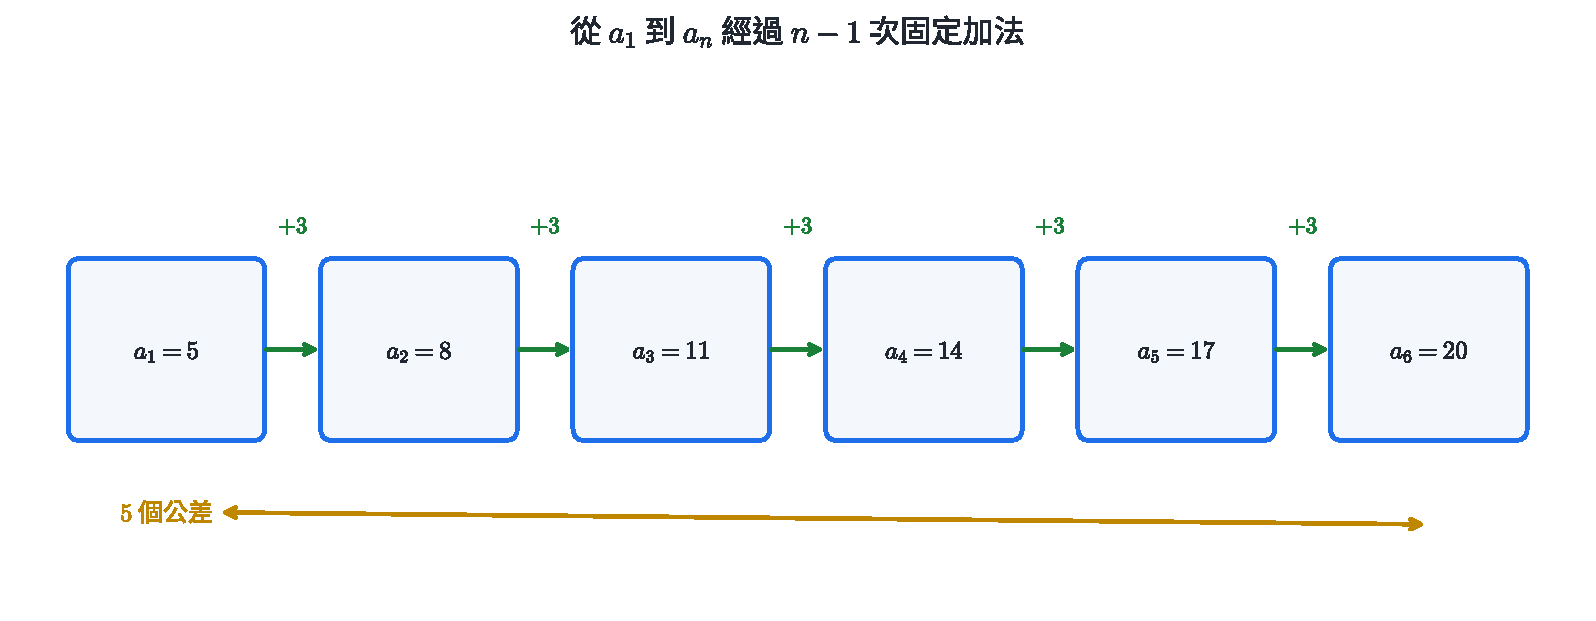
\includegraphics[width=0.92\linewidth,height=\textheight,keepaspectratio,alt={從第一項移到第六項，共累加五次公差}]{assets/數2-1-等差位移.pdf}
\caption{從第一項移到第六項，共累加五次公差}
\end{figure}

這個 \(n-1\) 直接來自步數。相鄰兩項相差一次，\(a_1\) 到 \(a_2\) 只有一步；同樣地，\(a_p\) 到 \(a_q\) 經過 \(q-p\) 步，所以

\[
a_q-a_p=(q-p)d.
\]

\subsection{例 3｜由兩個指定項決定等差數列}\label{ux4f8b-3ux7531ux5169ux500bux6307ux5b9aux9805ux6c7aux5b9aux7b49ux5deeux6578ux5217}

已知等差數列滿足 \(a_4=11\)、\(a_9=31\)，求通項。

兩個索引相差 \(5\)，因此

\[
a_9-a_4=5d
\quad\Longrightarrow\quad
31-11=5d,
\]

得 \(d=4\)。再由

\[
a_4=a_1+3d=11
\]

得 \(a_1=-1\)，所以

\[
\boxed{a_n=-1+4(n-1)=4n-5}.
\]

\subsection{例 4｜插入等差中項}\label{ux4f8b-4ux63d2ux5165ux7b49ux5deeux4e2dux9805}

在 \(8\) 與 \(32\) 之間插入 5 個數，使全部 7 個數成等差數列。

首尾之間有 \(7-1=6\) 段，因此

\[
d=\frac{32-8}{6}=4.
\]

數列為 \(8,12,16,20,24,28,32\)，插入的五個數是

\[
\boxed{12,16,20,24,28}.
\]

\subsection{2.2 等比數列：每一步乘固定倍率}\label{ux7b49ux6bd4ux6578ux5217ux6bcfux4e00ux6b65ux4e58ux56faux5b9aux500dux7387}

若 \(a_1\ne0\)，且數列從第二項起都滿足

\[
\frac{a_n}{a_{n-1}}=r,\qquad n\ge2,
\]

其中固定倍率 \(r\ne0\)，則稱為\textbf{等比數列}，\(r\) 稱為公比。從 \(a_1\) 到 \(a_n\) 共乘 \(n-1\) 次，故

\[
\boxed{a_n=a_1r^{n-1}}.
\]

\begin{figure}
\centering
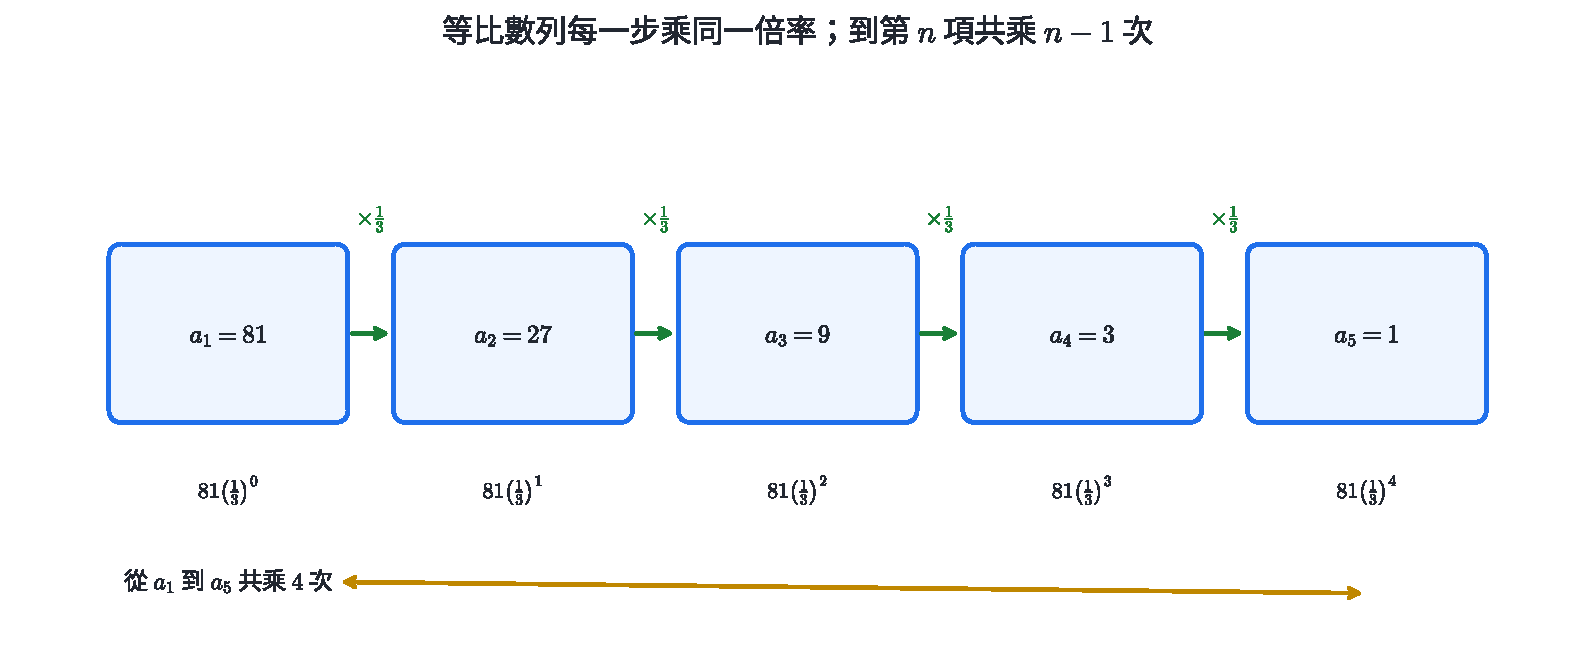
\includegraphics[width=0.92\linewidth,height=\textheight,keepaspectratio,alt={每一步乘三分之一，項值依序為 81、27、9、3、1}]{assets/數2-1-等比倍率.pdf}
\caption{每一步乘三分之一，項值依序為 81、27、9、3、1}
\end{figure}

公比可以為負數；此時各項正負交替。若只由相隔偶數步的兩項求公比，方程可能同時保留正、負兩種實數解。

\subsection{例 5｜相隔兩步的條件保留兩種公比}\label{ux4f8b-5ux76f8ux9694ux5169ux6b65ux7684ux689dux4ef6ux4fddux7559ux5169ux7a2eux516cux6bd4}

等比數列滿足 \(a_2=6\)、\(a_4=24\)，求所有可能的通項。

由 \(a_4=a_2r^2\) 得

\[
24=6r^2\quad\Longrightarrow\quad r^2=4,
\]

所以 \(r=2\) 或 \(r=-2\)。

\begin{itemize}
\tightlist
\item
  當 \(r=2\)，\(a_1=6/2=3\)，故 \(a_n=3\cdot2^{n-1}\)。
\item
  當 \(r=-2\)，\(a_1=6/(-2)=-3\)，故 \(a_n=-3(-2)^{n-1}\)。
\end{itemize}

兩個通項代入 \(n=2,4\) 都符合原條件。

\subsection{例 6｜固定保留率形成等比數列}\label{ux4f8b-6ux56faux5b9aux4fddux7559ux7387ux5f62ux6210ux7b49ux6bd4ux6578ux5217}

某訊號第一次量測為 \(640\) 單位，每經過一層材料後保留前一次的 \(1/2\)。第 \(n\) 次量測值為何？第 6 次是多少？

第一項為 \(640\)，公比為 \(1/2\)，所以

\[
a_n=640\left(\frac12\right)^{n-1}.
\]

第 6 次經過 5 次倍率更新：

\[
a_6=640\left(\frac12\right)^5=20.
\]

\subsection{2.3 分節練習}\label{ux5206ux7bc0ux7df4ux7fd2-1}

\begin{enumerate}
\def\labelenumi{\arabic{enumi}.}
\tightlist
\item
  等差數列 \(a_1=-7,d=5\)，求 \(a_{18}\)。
\item
  等差數列滿足 \(a_5=17,a_{12}=45\)，求 \(a_1,d,a_{30}\)。
\item
  在 \(-2\) 與 \(18\) 之間插入 3 個等差中項。
\item
  等比數列 \(a_1=5,r=-3\)，求 \(a_5,a_6\)。
\item
  等比數列滿足 \(a_3=12,a_6=96\)，求 \(a_1,r,a_8\)。
\item
  在 \(2\) 與 \(162\) 之間插入 3 個正數，使五個數成等比數列。
\end{enumerate}

\subsection{2.4 分節練習解析}\label{ux5206ux7bc0ux7df4ux7fd2ux89e3ux6790-1}

\begin{enumerate}
\def\labelenumi{\arabic{enumi}.}
\tightlist
\item
  \(a_{18}=-7+17(5)=78\)。
\item
  \(a_{12}-a_5=7d=28\)，故 \(d=4\)；\(a_1=17-4(4)=1\)；\(a_{30}=1+29(4)=117\)。
\item
  五個數之間有 4 段，\(d=[18-(-2)]/4=5\)，插入 \(3,8,13\)。
\item
  \(a_5=5(-3)^4=405\)，\(a_6=5(-3)^5=-1215\)。
\item
  \(a_6/a_3=r^3=8\)，故 \(r=2\)；\(a_1=12/2^2=3\)；\(a_8=3\cdot2^7=384\)。
\item
  設正公比為 \(r\)，則 \(2r^4=162\)，所以 \(r^4=81\) 且 \(r=3\)。插入 \(6,18,54\)。
\end{enumerate}

\section{3. 遞迴數列與數學歸納法}\label{ux905eux8ff4ux6578ux5217ux8207ux6578ux5b78ux6b78ux7d0dux6cd5}

\subsection{3.1 遞迴關係：由已知狀態產生下一項}\label{ux905eux8ff4ux95dcux4fc2ux7531ux5df2ux77e5ux72c0ux614bux7522ux751fux4e0bux4e00ux9805}

\textbf{遞迴數列}以初始值和更新規則共同定義。例如

\[
a_1=1,\qquad a_n=2a_{n-1}+1\quad(n\ge2)
\]

表示先固定 \(a_1\)，之後每一項都由前一項乘 2 再加 1。相同遞迴規則搭配不同初始值會產生不同數列，因此兩者都是完整定義的一部分。

\begin{figure}
\centering
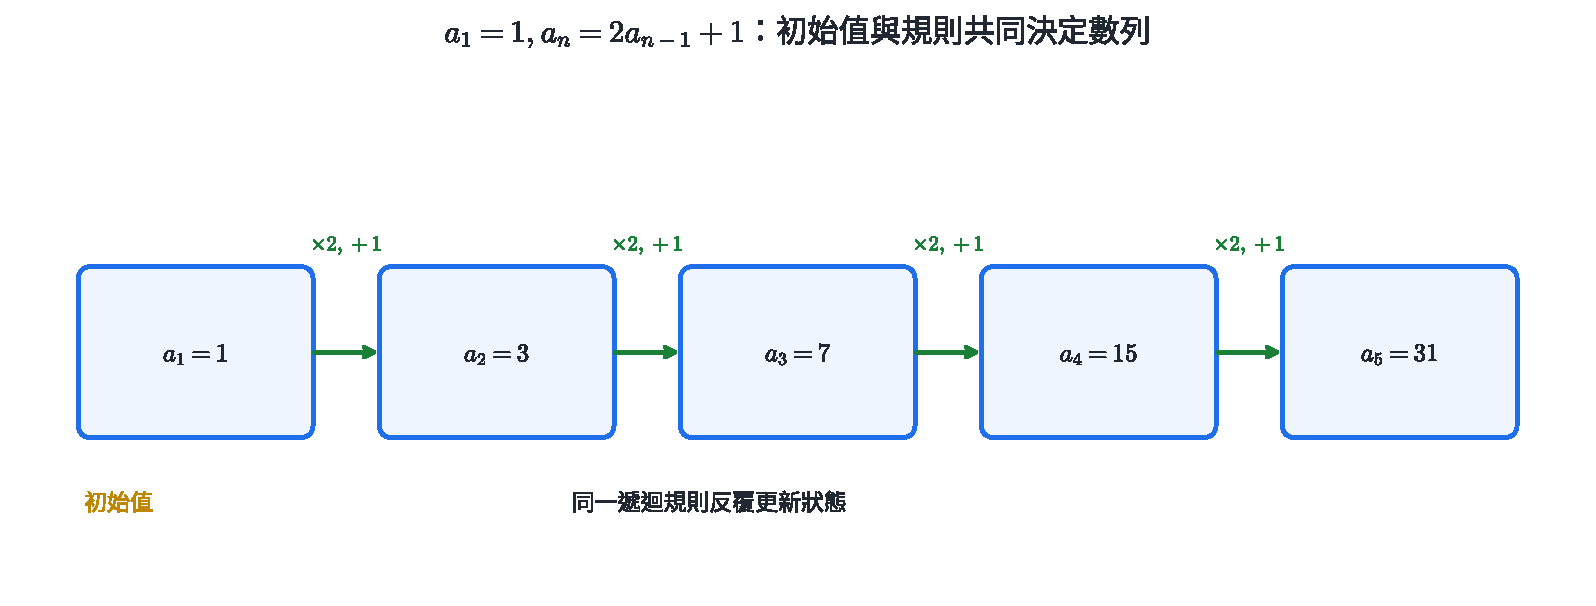
\includegraphics[width=0.92\linewidth,height=\textheight,keepaspectratio,alt={初始值 1 依同一規則更新為 3、7、15、31}]{assets/數2-1-遞迴狀態.pdf}
\caption{初始值 1 依同一規則更新為 3、7、15、31}
\end{figure}

等差與等比數列也可寫成遞迴形式：

\[
\text{等差： }a_n=a_{n-1}+d,\qquad
\text{等比： }a_n=ra_{n-1}.
\]

通項適合直接跳到第 \(n\) 項；遞迴式適合表達逐期更新、模擬狀態或由資料逐步生成下一項。

\subsection{例 7｜從遞迴式觀察並驗證通項}\label{ux4f8b-7ux5f9eux905eux8ff4ux5f0fux89c0ux5bdfux4e26ux9a57ux8b49ux901aux9805}

已知 \(a_1=1\)，\(a_n=2a_{n-1}+1\)。求前五項，並找出通項。

逐步更新得

\[
1,3,7,15,31.
\]

每一項都比相同索引的 \(2^n\) 少 1，因此猜測

\[
a_n=2^n-1.
\]

把它代回更新規則：

\[
2a_{n-1}+1=2(2^{n-1}-1)+1=2^n-1,
\]

並且 \(a_1=2^1-1=1\)，所以這個式子同時符合初始值與遞迴關係。

\subsection{例 8｜平移變數，把仿射遞迴化為等比}\label{ux4f8b-8ux5e73ux79fbux8b8aux6578ux628aux4effux5c04ux905eux8ff4ux5316ux70baux7b49ux6bd4}

已知 \(a_1=4\)，\(a_n=3a_{n-1}-2\)。求通項。

固定值 \(1\) 滿足 \(1=3(1)-2\)。令 \(b_n=a_n-1\)，則

\[
b_n=a_n-1=3a_{n-1}-3=3(a_{n-1}-1)=3b_{n-1}.
\]

又 \(b_1=3\)，所以 \(b_n=3\cdot3^{n-1}=3^n\)。因此

\[
\boxed{a_n=3^n+1}.
\]

這個平移的作用，是把「乘 3 再減 2」改寫成單純乘 3。

\subsection{3.2 數學歸納法：沿著正整數逐項證明}\label{ux6578ux5b78ux6b78ux7d0dux6cd5ux6cbfux8457ux6b63ux6574ux6578ux9010ux9805ux8b49ux660e}

設 \(P(n)\) 是關於正整數 \(n\) 的命題。若能完成

\begin{enumerate}
\def\labelenumi{\arabic{enumi}.}
\tightlist
\item
  \textbf{基礎步}：證明 \(P(1)\) 成立；
\item
  \textbf{歸納步}：對任意正整數 \(k\)，假設 \(P(k)\) 成立，並由此推出 \(P(k+1)\) 成立；
\end{enumerate}

便可判定 \(P(n)\) 對所有正整數 \(n\) 成立。

\begin{figure}
\centering
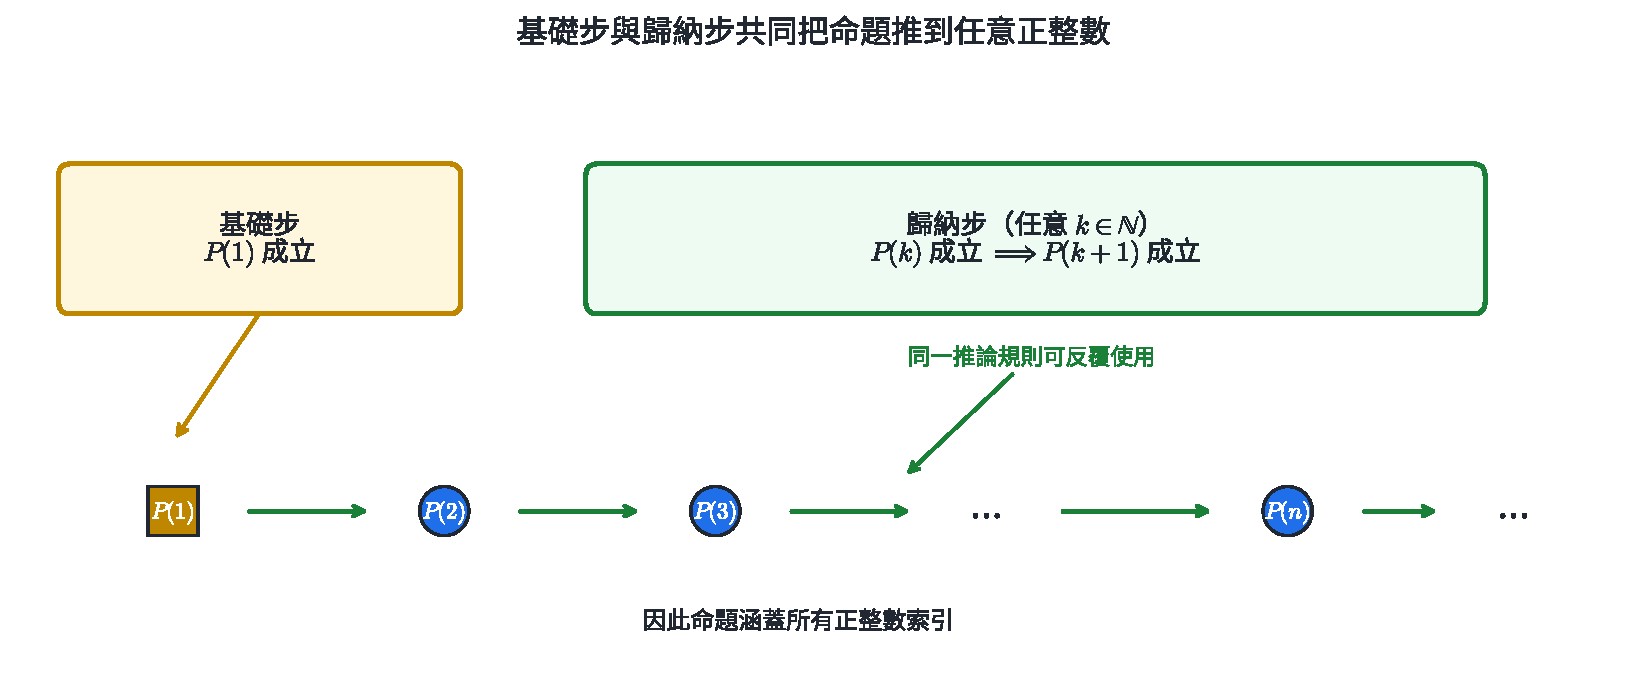
\includegraphics[width=0.94\linewidth,height=\textheight,keepaspectratio,alt={基礎步確立第一項，歸納步把任意一項的成立推到下一項}]{assets/數2-1-歸納法鏈條.pdf}
\caption{基礎步確立第一項，歸納步把任意一項的成立推到下一項}
\end{figure}

歸納步中的 \(k\) 代表任意已到達的位置。推導必須實際使用歸納假設，才能把 \(P(k)\) 與 \(P(k+1)\) 接起來。

\subsection{\texorpdfstring{例 9｜證明前 \(n\) 個奇數的和}{例 9｜證明前 n 個奇數的和}}\label{ux4f8b-9ux8b49ux660eux524d-n-ux500bux5947ux6578ux7684ux548c}

證明對所有正整數 \(n\)，

\[
1+3+5+\cdots+(2n-1)=n^2.
\]

\textbf{基礎步。} \(n=1\) 時，左式 \(=1\)，右式 \(=1^2\)，命題成立。

\textbf{歸納步。} 假設 \(n=k\) 時成立，即

\[
1+3+\cdots+(2k-1)=k^2.
\]

則 \(n=k+1\) 時，左式多出下一個奇數 \(2k+1\)：

\[
1+3+\cdots+(2k-1)+(2k+1)
=k^2+2k+1=(k+1)^2.
\]

所以命題對所有正整數 \(n\) 成立。

\subsection{例 10｜用歸納法證明遞迴數列的通項}\label{ux4f8b-10ux7528ux6b78ux7d0dux6cd5ux8b49ux660eux905eux8ff4ux6578ux5217ux7684ux901aux9805}

對 \(a_1=1\)、\(a_n=2a_{n-1}+1\)，證明 \(a_n=2^n-1\)。

\textbf{基礎步。} \(a_1=1=2^1-1\)。

\textbf{歸納步。} 假設 \(a_k=2^k-1\)，由遞迴式

\[
a_{k+1}=2a_k+1=2(2^k-1)+1=2^{k+1}-1.
\]

因此通項對所有正整數 \(n\) 成立。

\subsection{3.3 分節練習}\label{ux5206ux7bc0ux7df4ux7fd2-2}

\begin{enumerate}
\def\labelenumi{\arabic{enumi}.}
\tightlist
\item
  \(a_1=a_2=1\)，\(a_n=a_{n-1}+a_{n-2}\)（\(n\ge3\)）。寫出前七項。
\item
  \(a_1=2\)，\(a_n=a_{n-1}+3n\)（\(n\ge2\)）。求 \(a_2\) 至 \(a_5\)。
\item
  \(c_1=5\)，\(c_n=2c_{n-1}-3\)。以適當平移求通項。
\item
  用數學歸納法證明 \(1+2+\cdots+n=\dfrac{n(n+1)}2\)。
\item
  用數學歸納法證明 \(3^n\ge2n+1\) 對所有正整數 \(n\) 成立。
\item
  用數學歸納法證明 \(7^n-1\) 可被 \(6\) 整除。
\end{enumerate}

\subsection{3.4 分節練習解析}\label{ux5206ux7bc0ux7df4ux7fd2ux89e3ux6790-2}

\begin{enumerate}
\def\labelenumi{\arabic{enumi}.}
\tightlist
\item
  每一項等於前兩項之和，依序為 \(1,1,2,3,5,8,13\)。
\item
  \(a_2=2+6=8\)，\(a_3=8+9=17\)，\(a_4=17+12=29\)，\(a_5=29+15=44\)。
\item
  固定值為 \(3\)。令 \(b_n=c_n-3\)，則 \(b_n=2b_{n-1}\)，且 \(b_1=2\)，故 \(b_n=2^n\)，\(\boxed{c_n=2^n+3}\)。
\item
  \(n=1\) 時成立。假設 \(1+\cdots+k=k(k+1)/2\)，則
  \[
  1+\cdots+k+(k+1)=\frac{k(k+1)}2+(k+1)=\frac{(k+1)(k+2)}2,
  \]
  正是 \(n=k+1\) 的式子。
\item
  \(n=1\) 時 \(3=3\)。假設 \(3^k\ge2k+1\)，則
  \[
  3^{k+1}\ge3(2k+1)=6k+3\ge2k+3=2(k+1)+1.
  \]
\item
  \(n=1\) 時 \(7-1=6\)。假設 \(7^k-1=6m\)，則
  \[
  7^{k+1}-1=7(7^k-1)+6=6(7m+1),
  \]
  因此仍可被 \(6\) 整除。
\end{enumerate}

\section{4. 有限級數、等差和與等比和}\label{ux6709ux9650ux7d1aux6578ux7b49ux5deeux548cux8207ux7b49ux6bd4ux548c}

\subsection{4.1 級數與部分和}\label{ux7d1aux6578ux8207ux90e8ux5206ux548c}

把數列的前 \(n\) 項相加所得的式子

\[
a_1+a_2+\cdots+a_n
\]

稱為\textbf{有限級數}，其和記作

\[
S_n=a_1+a_2+\cdots+a_n=\sum_{k=1}^{n}a_k.
\]

\(\sum\) 是求和符號，\(k\) 是求和索引。下限 \(1\) 與上限 \(n\) 決定實際相加的項，總共有 \(n\) 項。當 \(n\) 依序取 \(1,2,3,\ldots\) 時，\(S_1,S_2,S_3,\ldots\) 本身也形成一個數列，稱為部分和數列。

\begin{figure}
\centering
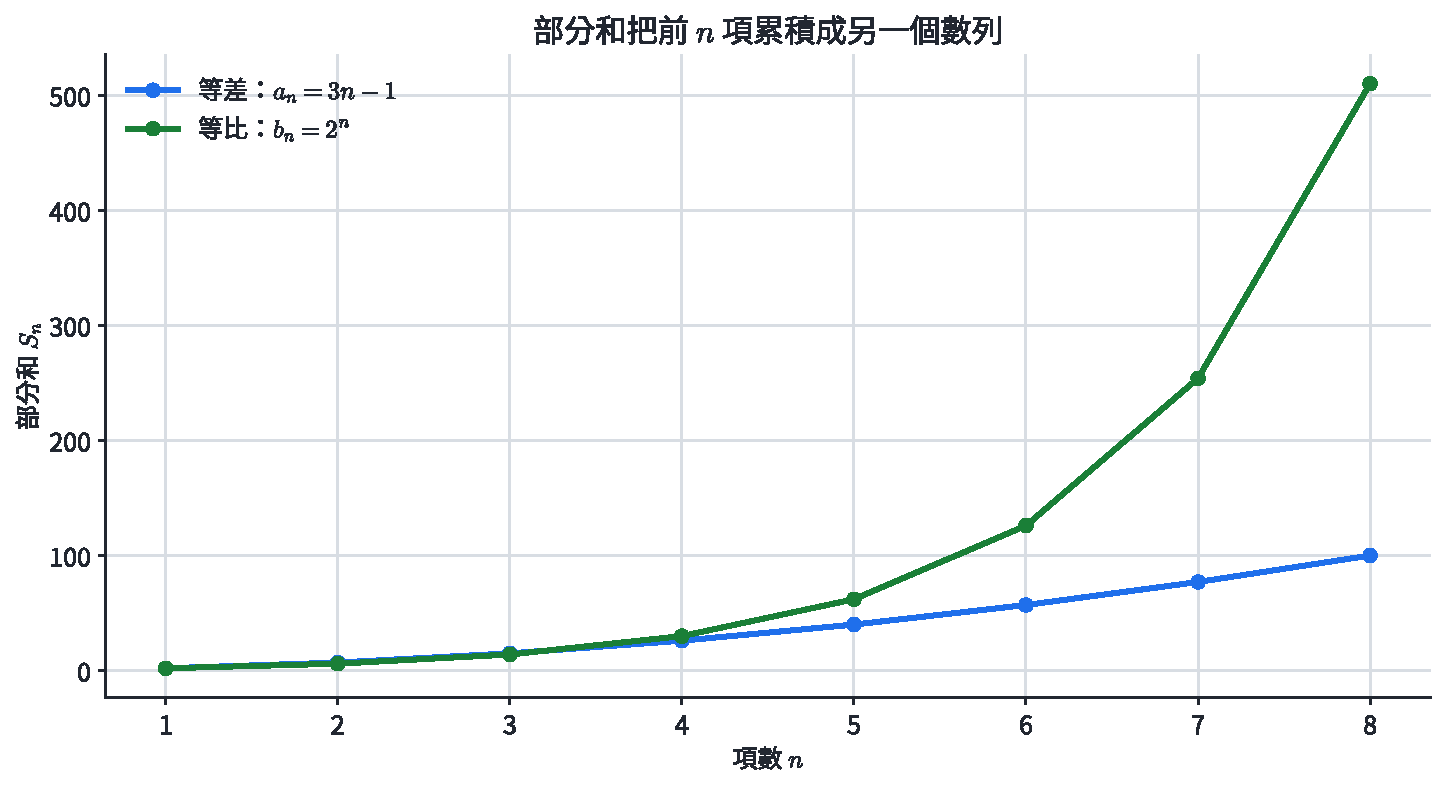
\includegraphics[width=0.88\linewidth,height=\textheight,keepaspectratio,alt={等差與等比數列的部分和均由逐項累積得到，但成長尺度不同}]{assets/數2-1-部分和成長.pdf}
\caption{等差與等比數列的部分和均由逐項累積得到，但成長尺度不同}
\end{figure}

由定義直接得到

\[
S_n=S_{n-1}+a_n\quad(n\ge2),
\]

所以

\[
a_1=S_1,\qquad a_n=S_n-S_{n-1}\quad(n\ge2).
\]

前一式用來累積，後一式用相鄰兩個累積量還原單期增量。

\subsection{4.2 等差級數：首尾配對}\label{ux7b49ux5deeux7d1aux6578ux9996ux5c3eux914dux5c0d}

設等差數列前 \(n\) 項和為

\[
S_n=a_1+a_2+\cdots+a_n.
\]

將相同級數倒序寫一次：

\[
S_n=a_n+a_{n-1}+\cdots+a_1.
\]

上下相加後，每一欄都是 \(a_1+a_n\)，共有 \(n\) 欄，因此

\[
2S_n=n(a_1+a_n).
\]

故

\[
\boxed{S_n=\frac{n(a_1+a_n)}2
=\frac n2\left[2a_1+(n-1)d\right]}.
\]

\begin{figure}
\centering
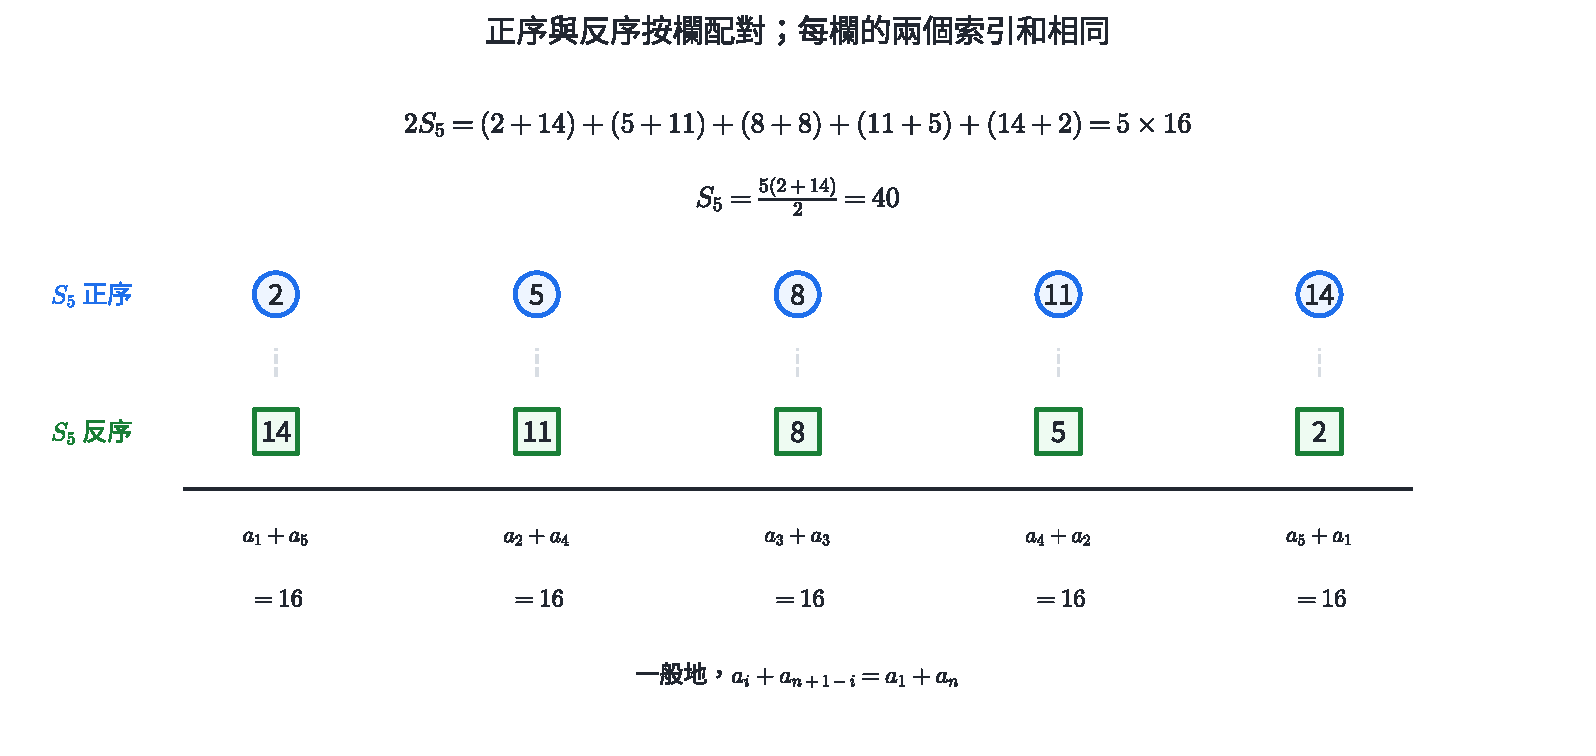
\includegraphics[width=0.9\linewidth,height=\textheight,keepaspectratio,alt={等差級數正序與反序按欄配對，第 i 欄滿足 a\_i 加 a\_\{n+1-i\} 等於首項加末項}]{assets/數2-1-等差級數配對.pdf}
\caption{等差級數正序與反序按欄配對，第 i 欄滿足 a\_i 加 a\_\{n+1-i\} 等於首項加末項}
\end{figure}

\subsection{例 11｜先由首尾求項數，再求和}\label{ux4f8b-11ux5148ux7531ux9996ux5c3eux6c42ux9805ux6578ux518dux6c42ux548c}

求

\[
7+11+15+\cdots+39.
\]

首項 \(a_1=7\)，公差 \(d=4\)。由

\[
39=7+(n-1)4
\]

得 \(n=9\)。因此

\[
S_9=\frac{9(7+39)}2=207.
\]

首尾差 \(32\) 對應 8 個公差，因此共有 9 項。

\subsection{例 12｜由兩項條件建立整個級數}\label{ux4f8b-12ux7531ux5169ux9805ux689dux4ef6ux5efaux7acbux6574ux500bux7d1aux6578}

等差數列滿足 \(a_3=8\)、\(a_{10}=29\)，求 \(S_{20}\)。

兩項相隔 7 步：

\[
29-8=7d\quad\Longrightarrow\quad d=3.
\]

故 \(a_1=8-2(3)=2\)，\(a_{20}=2+19(3)=59\)。所以

\[
S_{20}=\frac{20(2+59)}2=610.
\]

\subsection{4.3 等比級數：乘公比後錯位相減}\label{ux7b49ux6bd4ux7d1aux6578ux4e58ux516cux6bd4ux5f8cux932fux4f4dux76f8ux6e1b}

設

\[
S_n=a_1+a_1r+a_1r^2+\cdots+a_1r^{n-1}.
\]

兩邊乘 \(r\)：

\[
rS_n=a_1r+a_1r^2+\cdots+a_1r^{n-1}+a_1r^n.
\]

相減後中間各項消去：

\[
S_n-rS_n=a_1-a_1r^n.
\]

當 \(r\ne1\) 時，可除以 \(1-r\)：

\[
\boxed{S_n=\frac{a_1(1-r^n)}{1-r}}
\qquad(r\ne1).
\]

當 \(r=1\) 時，每一項都是 \(a_1\)，因此

\[
\boxed{S_n=na_1}.
\]

\begin{figure}
\centering
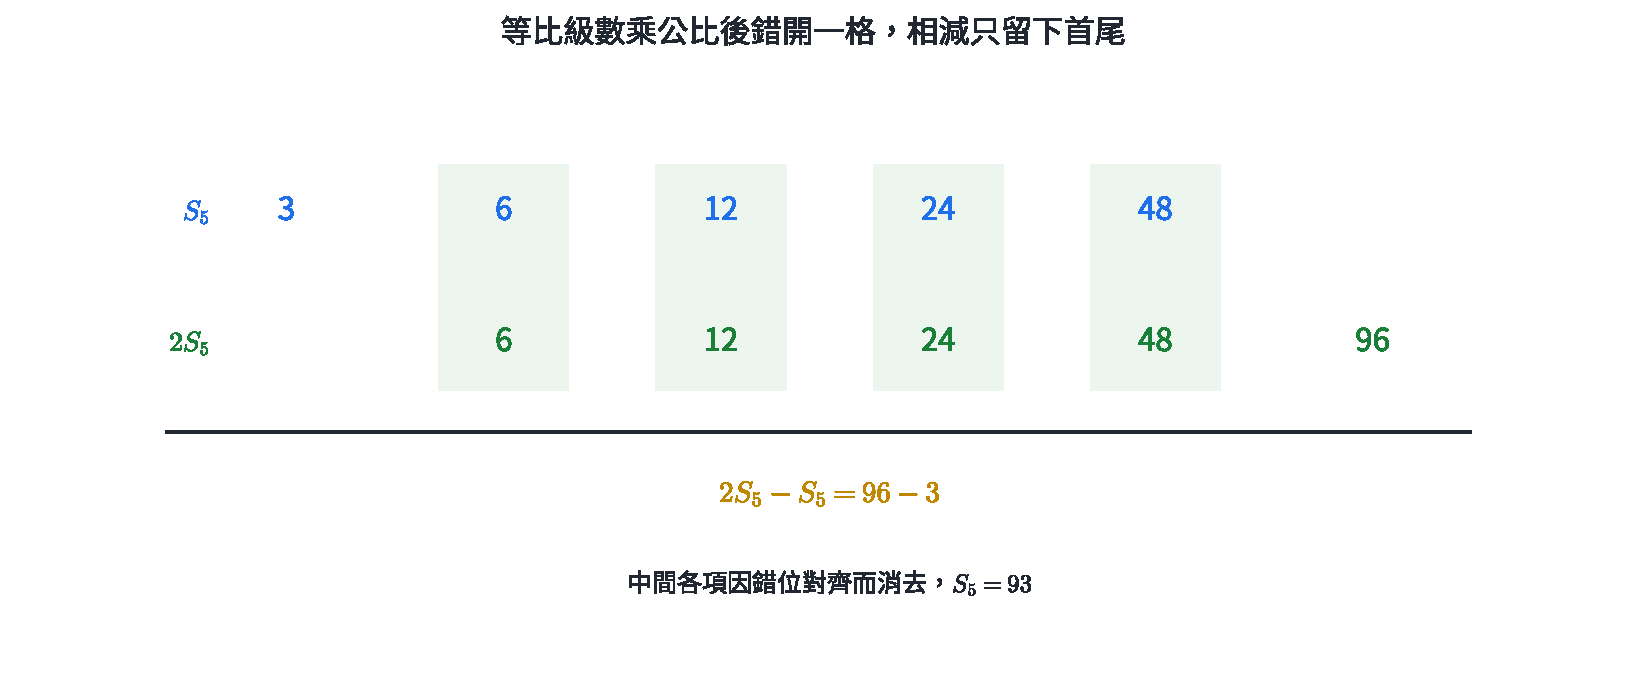
\includegraphics[width=0.92\linewidth,height=\textheight,keepaspectratio,alt={以公比 2 乘整個級數後錯開一格，相減留下首項與新尾項}]{assets/數2-1-等比級數錯位相減.pdf}
\caption{以公比 2 乘整個級數後錯開一格，相減留下首項與新尾項}
\end{figure}

\subsection{例 13｜公比為負的有限等比級數}\label{ux4f8b-13ux516cux6bd4ux70baux8ca0ux7684ux6709ux9650ux7b49ux6bd4ux7d1aux6578}

求 \(3-6+12-24+48-96\)。

這是 \(a_1=3\)、\(r=-2\)、\(n=6\) 的等比級數：

\[
S_6=\frac{3[1-(-2)^6]}{1-(-2)}
=\frac{3(1-64)}3=-63.
\]

直接估計也合理：最後一項為 \(-96\)，前五項和為 \(33\)，總和為負。

\subsection{例 14｜由級數總和反求項數}\label{ux4f8b-14ux7531ux7d1aux6578ux7e3dux548cux53cdux6c42ux9805ux6578}

已知

\[
5+10+20+\cdots+5\cdot2^{n-1}=1275,
\]

求 \(n\)。

左式是 \(a_1=5,r=2\) 的前 \(n\) 項和：

\[
5\frac{1-2^n}{1-2}=5(2^n-1)=1275.
\]

所以 \(2^n=256=2^8\)，故 \(n=8\)。

\subsection{4.4 分節練習}\label{ux5206ux7bc0ux7df4ux7fd2-3}

\begin{enumerate}
\def\labelenumi{\arabic{enumi}.}
\tightlist
\item
  求 \(4+7+10+\cdots+61\)。
\item
  等差數列滿足 \(a_7=20,d=-2\)，求 \(S_{15}\)。
\item
  求 \(2+6+18+\cdots+4374\)。
\item
  求 \(10-5+2.5-\cdots\) 的前 8 項和。
\item
  等比數列的公比為 \(1\)、首項為 \(7\)，求前 30 項和。
\item
  已知 \(3+6+12+\cdots+3\cdot2^{n-1}=3069\)，求 \(n\)。
\end{enumerate}

\subsection{4.5 分節練習解析}\label{ux5206ux7bc0ux7df4ux7fd2ux89e3ux6790-3}

\begin{enumerate}
\def\labelenumi{\arabic{enumi}.}
\tightlist
\item
  \(61=4+(n-1)3\)，得 \(n=20\)；\(S_{20}=20(4+61)/2=650\)。
\item
  \(a_1=a_7-6d=20-6(-2)=32\)，\(a_{15}=32+14(-2)=4\)，故 \(S_{15}=15(32+4)/2=270\)。
\item
  \(4374=2\cdot3^7\)，所以共有 8 項；
  \[
  S_8=\frac{2(1-3^8)}{1-3}=6560.
  \]
\item
  \(a_1=10,r=-1/2,n=8\)，故
  \[
  S_8=\frac{10[1-(-1/2)^8]}{1+1/2}=\frac{425}{64}\approx6.641.
  \]
\item
  \(r=1\) 時每項均為 \(7\)，\(S_{30}=30\cdot7=210\)。
\item
  \(3(2^n-1)=3069\)，得 \(2^n=1024=2^{10}\)，所以 \(n=10\)。
\end{enumerate}

\section{5. 常用和式、拆項與由部分和還原數列}\label{ux5e38ux7528ux548cux5f0fux62c6ux9805ux8207ux7531ux90e8ux5206ux548cux9084ux539fux6578ux5217}

\subsection{5.1 三個常用有限和}\label{ux4e09ux500bux5e38ux7528ux6709ux9650ux548c}

對正整數 \(n\)，有

\[
\sum_{k=1}^{n}k=\frac{n(n+1)}2,
\]

\[
\sum_{k=1}^{n}k^2=\frac{n(n+1)(2n+1)}6,
\]

\[
\sum_{k=1}^{n}k^3=\left[\frac{n(n+1)}2\right]^2.
\]

第一式是首項 \(1\)、末項 \(n\) 的等差級數公式。後兩式可用數學歸納法驗證。例如，若平方和公式在 \(n=k\) 成立，加入 \((k+1)^2\) 後：

\[
\frac{k(k+1)(2k+1)}6+(k+1)^2
=\frac{(k+1)(k+2)(2k+3)}6,
\]

正是把 \(n\) 換成 \(k+1\) 的公式。立方和的歸納步則為

\[
\left[\frac{k(k+1)}2\right]^2+(k+1)^3
=\left[\frac{(k+1)(k+2)}2\right]^2.
\]

\subsection{5.2 求和的線性與拆項}\label{ux6c42ux548cux7684ux7ddaux6027ux8207ux62c6ux9805}

同一求和範圍內，可逐項使用分配律：

\[
\sum_{k=1}^{n}[c,u_k+d,v_k]
=c\sum_{k=1}^{n}u_k+d\sum_{k=1}^{n}v_k.
\]

因此多項式型的一般項可展開後，分別套用一次、平方、立方和公式。

\begin{figure}
\centering
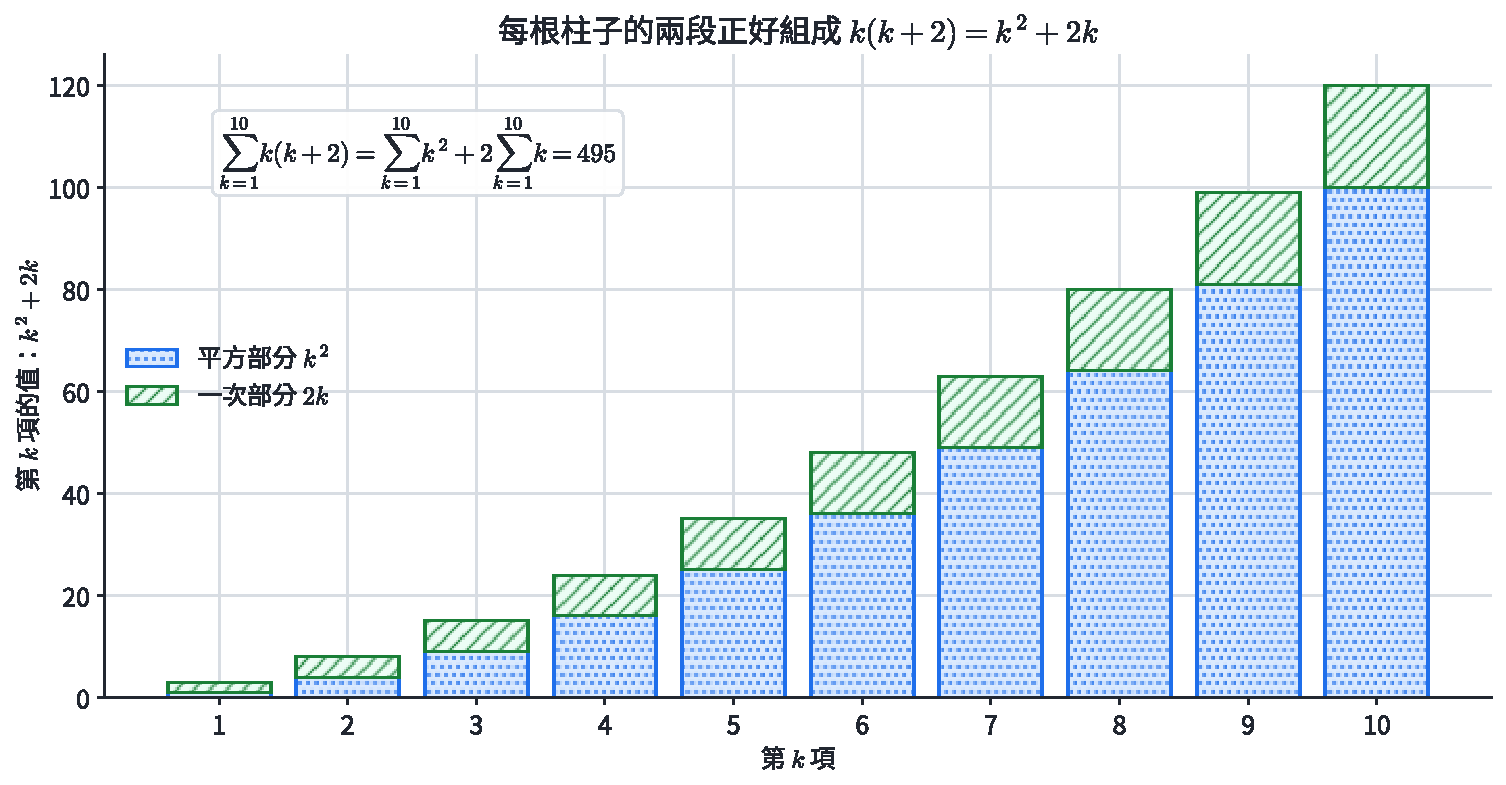
\includegraphics[width=0.88\linewidth,height=\textheight,keepaspectratio,alt={每個 k(k+2) 拆成 k 平方與 2k，總和也可分開計算}]{assets/數2-1-拆項求和.pdf}
\caption{每個 k(k+2) 拆成 k 平方與 2k，總和也可分開計算}
\end{figure}

\subsection{例 15｜拆成平方和與一次和}\label{ux4f8b-15ux62c6ux6210ux5e73ux65b9ux548cux8207ux4e00ux6b21ux548c}

求

\[
\sum_{k=1}^{10}k(k+2).
\]

先展開 \(k(k+2)=k^2+2k\)：

\[
\begin{aligned}
\sum_{k=1}^{10}k(k+2)
&=\sum_{k=1}^{10}k^2+2\sum_{k=1}^{10}k\\
&=\frac{10\cdot11\cdot21}{6}
+2\cdot\frac{10\cdot11}{2}\\
&=385+110=495.
\end{aligned}
\]

\subsection{例 16｜展開後處理奇數平方和}\label{ux4f8b-16ux5c55ux958bux5f8cux8655ux7406ux5947ux6578ux5e73ux65b9ux548c}

求 \(\displaystyle\sum_{k=1}^{8}(2k-1)^2\)。

因為 \((2k-1)^2=4k^2-4k+1\)，所以

\[
\begin{aligned}
\sum_{k=1}^{8}(2k-1)^2
&=4\sum_{k=1}^{8}k^2-4\sum_{k=1}^{8}k+\sum_{k=1}^{8}1\\
&=4(204)-4(36)+8\\
&=680.
\end{aligned}
\]

最後一項 \(\sum_{k=1}^{8}1=8\)，因為常數 \(1\) 共出現 8 次。

\subsection{\texorpdfstring{5.3 由 \(S_n\) 求 \(a_n\)}{5.3 由 S\_n 求 a\_n}}\label{ux7531-s_n-ux6c42-a_n}

\(S_n\) 是前 \(n\) 項累積量。相鄰部分和相減時，前 \(n-1\) 項全部消去，留下第 \(n\) 項：

\[
S_n-S_{n-1}=a_n\qquad(n\ge2).
\]

第一項需由 \(a_1=S_1\) 取得，再檢查求出的 \(n\ge2\) 公式是否也適用於 \(n=1\)。

\subsection{例 17｜從二次部分和還原一次通項}\label{ux4f8b-17ux5f9eux4e8cux6b21ux90e8ux5206ux548cux9084ux539fux4e00ux6b21ux901aux9805}

已知 \(S_n=2n^2\)，求 \(a_n\)。

第一項為

\[
a_1=S_1=2.
\]

對 \(n\ge2\)，

\[
\begin{aligned}
a_n&=S_n-S_{n-1}\\
&=2n^2-2(n-1)^2\\
&=4n-2.
\end{aligned}
\]

把 \(n=1\) 代入 \(4n-2\) 也得 \(2\)，所以可統一寫成

\[
\boxed{a_n=4n-2\quad(n\ge1)}.
\]

\subsection{例 18｜逐層增加的材料總量}\label{ux4f8b-18ux9010ux5c64ux589eux52a0ux7684ux6750ux6599ux7e3dux91cf}

第 \(k\) 層使用 \(3k-2\) 個元件。求前 20 層總數。

\[
\begin{aligned}
S_{20}
&=\sum_{k=1}^{20}(3k-2)\\
&=3\sum_{k=1}^{20}k-2\sum_{k=1}^{20}1\\
&=3\cdot\frac{20\cdot21}{2}-2(20)\\
&=590.
\end{aligned}
\]

這裡的常數項 \(-2\) 在每一層都出現一次，因此總貢獻是 \(-2\times20\)。

\subsection{5.4 分節練習}\label{ux5206ux7bc0ux7df4ux7fd2-4}

\begin{enumerate}
\def\labelenumi{\arabic{enumi}.}
\tightlist
\item
  求 \(\displaystyle\sum_{k=1}^{25}k\)。
\item
  求 \(\displaystyle\sum_{k=1}^{12}k^2\)。
\item
  求 \(\displaystyle\sum_{k=1}^{8}k^3\)。
\item
  求 \(\displaystyle\sum_{k=1}^{10}k(2k-1)\)。
\item
  已知 \(S_n=n^2+4n\)，求 \(a_n\) 與 \(a_{15}\)。
\end{enumerate}

\subsection{5.5 分節練習解析}\label{ux5206ux7bc0ux7df4ux7fd2ux89e3ux6790-4}

\begin{enumerate}
\def\labelenumi{\arabic{enumi}.}
\tightlist
\item
  \(25\cdot26/2=325\)。
\item
  \(12\cdot13\cdot25/6=650\)。
\item
  \([8\cdot9/2]^2=36^2=1296\)。
\item
  \(k(2k-1)=2k^2-k\)，故總和為 \(2(385)-55=715\)。
\item
  \(a_1=S_1=5\)。對 \(n\ge2\)，
  \[
  a_n=(n^2+4n)-[(n-1)^2+4(n-1)]=2n+3.
  \]
  這個式子在 \(n=1\) 也給出 \(5\)，故 \(a_n=2n+3\)，\(a_{15}=33\)。
\end{enumerate}

\section{6. 單利、複利與定期存款}\label{ux55aeux5229ux8907ux5229ux8207ux5b9aux671fux5b58ux6b3e}

\subsection{6.1 單利與複利的更新機制}\label{ux55aeux5229ux8207ux8907ux5229ux7684ux66f4ux65b0ux6a5fux5236}

設本金為 \(P\)，每期利率為 \(r\)，經過 \(n\) 期。

\textbf{單利}每一期都只按原始本金計息，每期增加 \(Pr\)：

\[
A_n=P+nPr=P(1+nr).
\]

\textbf{複利}把前一期本利和作為下一期本金，每期乘 \(1+r\)：

\[
A_n=P(1+r)^n.
\]

\begin{figure}
\centering
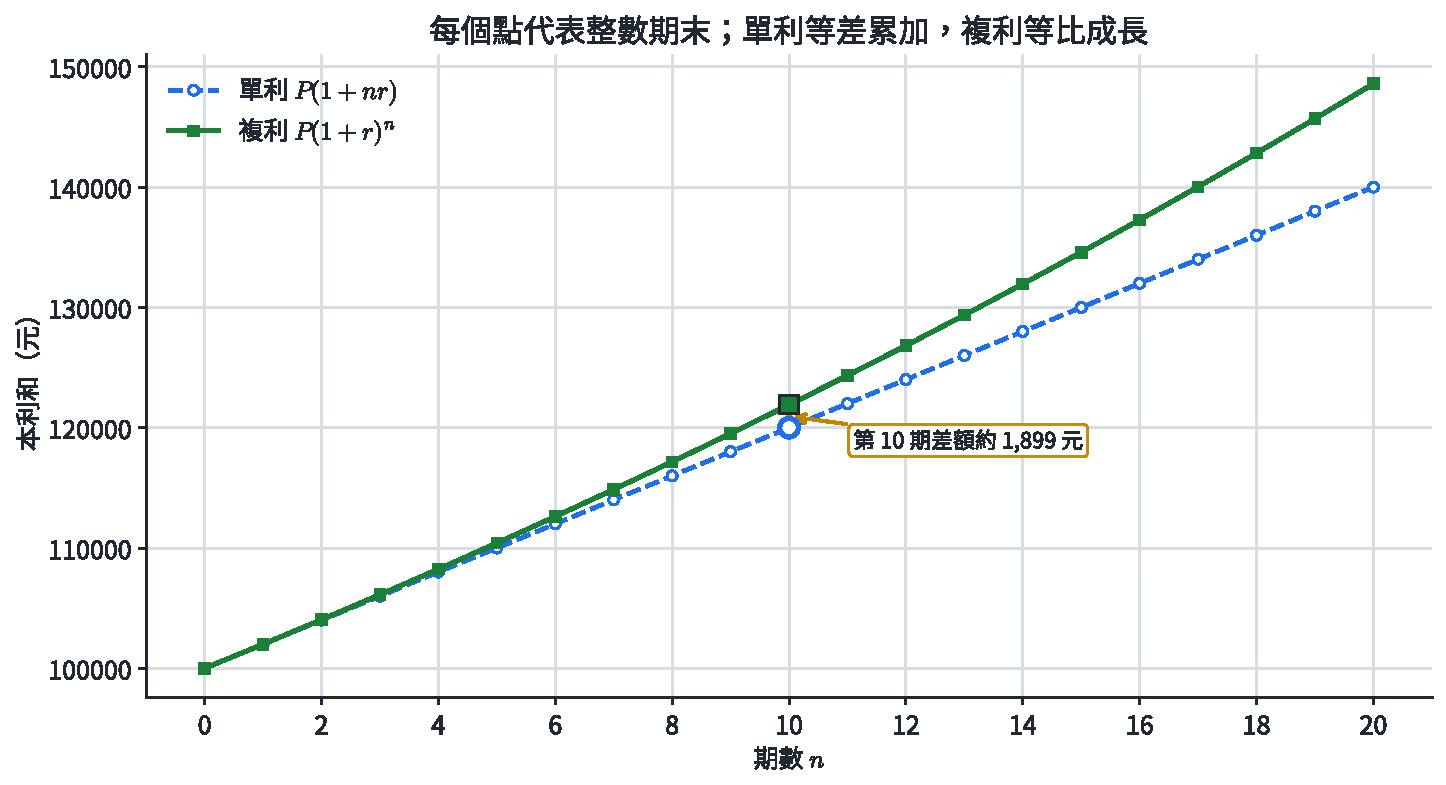
\includegraphics[width=0.88\linewidth,height=\textheight,keepaspectratio,alt={十萬元在固定 2\% 期利率下，各整數期末的單利金額呈等差累加，複利金額呈等比成長}]{assets/數2-1-單利複利比較.pdf}
\caption{十萬元在固定 2\% 期利率下，各整數期末的單利金額呈等差累加，複利金額呈等比成長}
\end{figure}

利率與期數必須使用同一時間單位。例如月利率搭配月數，年利率搭配年數。固定利率模型提供基準估算；實際金融商品還可能含手續費、稅、浮動利率與不同計息規則。

\subsection{例 19｜比較同一條件下的單利與複利}\label{ux4f8b-19ux6bd4ux8f03ux540cux4e00ux689dux4ef6ux4e0bux7684ux55aeux5229ux8207ux8907ux5229}

本金 \(100000\) 元，每期利率 \(2\%\)，共 10 期。

單利本利和：

\[
A_{10}=100000[1+10(0.02)]=120000.
\]

複利本利和：

\[
A_{10}=100000(1.02)^{10}\approx121899.44.
\]

複利多約 \(1899.44\) 元，差額來自先前利息也參與後續計息。

\subsection{6.2 每期初固定存款的終值}\label{ux6bcfux671fux521dux56faux5b9aux5b58ux6b3eux7684ux7d42ux503c}

每期初存入 \(P\) 元，期利率為 \(r\)，共存 \(N\) 次，並在第 \(N\) 期期末結算。第一次存款計息 \(N\) 期，最後一次存款計息 1 期，因此各筆終值依序為

\[
P(1+r)^N,P(1+r)^{N-1},\ldots,P(1+r).
\]

\begin{figure}
\centering
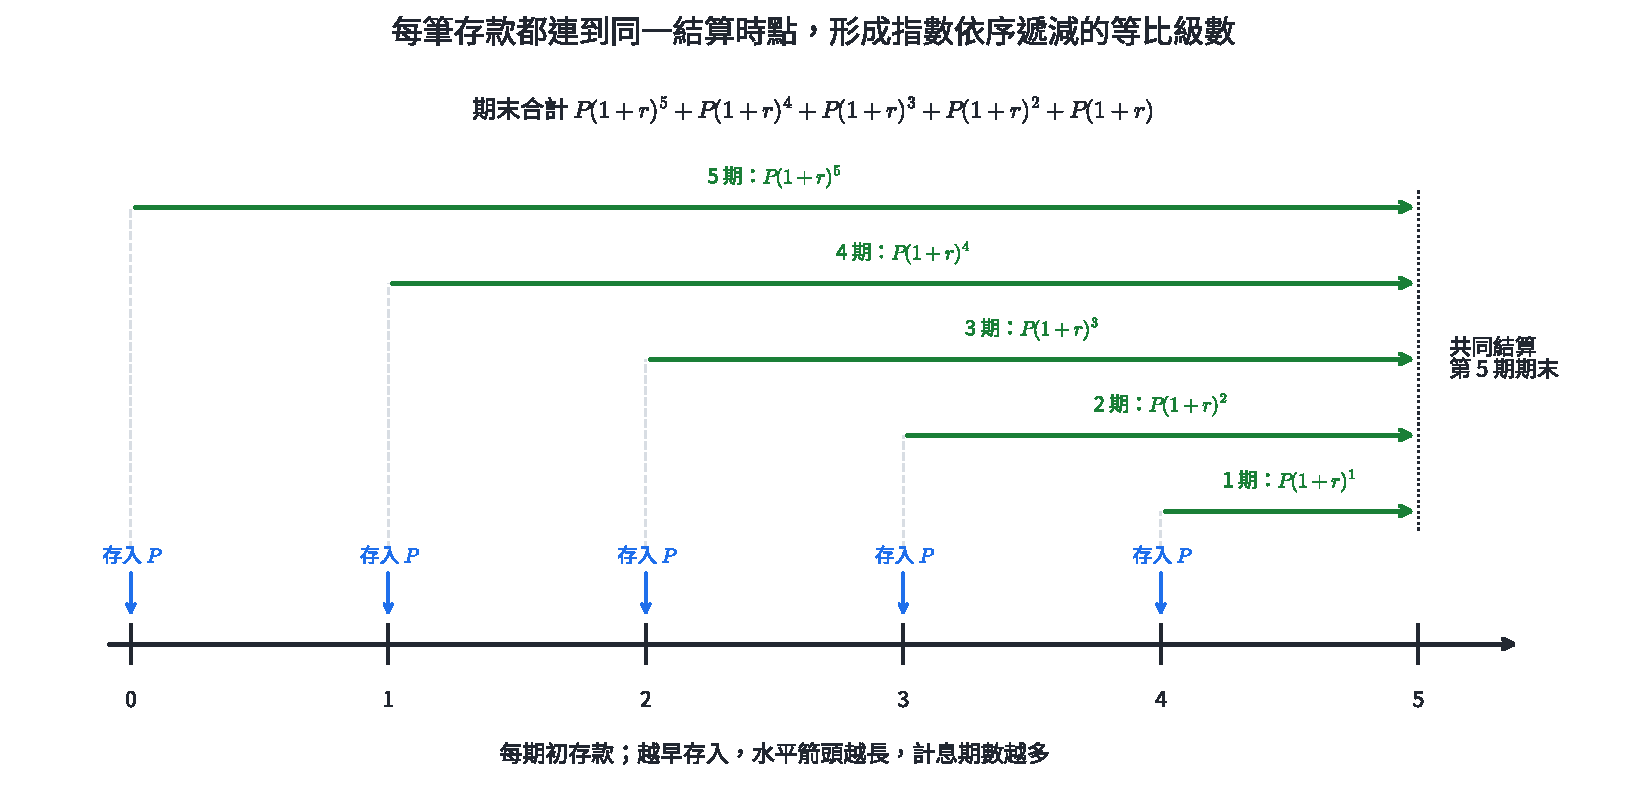
\includegraphics[width=0.94\linewidth,height=\textheight,keepaspectratio,alt={每期初存款到共同結算時點的計息期數依序遞減}]{assets/數2-1-定期存款時間軸.pdf}
\caption{每期初存款到共同結算時點的計息期數依序遞減}
\end{figure}

令 \(q=1+r\)。當 \(r\ne0\) 時，期末總額為

\[
\begin{aligned}
F_N
&=P(q+q^2+\cdots+q^N)\\
&=\boxed{Pq\frac{q^N-1}{q-1}}
=\boxed{P(1+r)\frac{(1+r)^N-1}{r}}.
\end{aligned}
\]

當 \(r=0\) 時，每筆存款維持原值，總額為 \(NP\)。若改成每期期末存入，最後一筆在結算時尚未計息，指數會改為 \(N-1,N-2,\ldots,0\)。

\subsection{例 20｜十二次月初存款的期末總額}\label{ux4f8b-20ux5341ux4e8cux6b21ux6708ux521dux5b58ux6b3eux7684ux671fux672bux7e3dux984d}

每月初存入 \(10000\) 元，月利率 \(0.1\%=0.001\)，連續存 12 次，在第 12 個月底結算。

第一筆有 12 個月利息，最後一筆有 1 個月利息：

\[
F_{12}=10000(1.001)\frac{(1.001)^{12}-1}{0.001}
\approx120782.87.
\]

總投入為 \(120000\) 元，因此利息約為 \(782.87\) 元。

\subsection{例 21｜固定保留率的設備價值}\label{ux4f8b-21ux56faux5b9aux4fddux7559ux7387ux7684ux8a2dux5099ux50f9ux503c}

設備購入價為 \(300000\) 元，每年末估值為前一年的 \(85\%\)。四年後的模型估值為

\[
V_4=300000(0.85)^4\approx156601.88\text{ 元}.
\]

每年保留率固定，故價值形成公比 \(0.85\) 的等比變化。這是估值模型；實際售價還受市場、維修與使用狀況影響。

\subsection{6.3 分節練習}\label{ux5206ux7bc0ux7df4ux7fd2-5}

\begin{enumerate}
\def\labelenumi{\arabic{enumi}.}
\tightlist
\item
  本金 \(200000\) 元，以每年 \(3\%\) 複利計算 5 年，求本利和。
\item
  本金 \(80000\) 元，以每期 \(1.2\%\) 單利計算 8 期，求本利和。
\item
  本金 \(50000\) 元，以每月 \(1\%\) 複利計算 12 個月，求本利和。
\item
  每月初存入 \(5000\) 元，月利率 \(0.5\%\)，連續存 24 次，在第 24 個月底結算，求總額。
\item
  一項設備每年保留前一年價值的 \(85\%\)，原價 \(300000\) 元，求四年後的模型估值。
\end{enumerate}

\subsection{6.4 分節練習解析}\label{ux5206ux7bc0ux7df4ux7fd2ux89e3ux6790-5}

\begin{enumerate}
\def\labelenumi{\arabic{enumi}.}
\tightlist
\item
  \(200000(1.03)^5\approx231854.81\) 元。
\item
  \(80000[1+8(0.012)]=87680\) 元。
\item
  \(50000(1.01)^{12}\approx56341.25\) 元。
\item
  月初存款在結算時的指數為 \(24,23,\ldots,1\)：
  \[
  F=5000(1.005)\frac{(1.005)^{24}-1}{0.005}\approx127795.58\text{ 元}.
  \]
\item
  \(300000(0.85)^4\approx156601.88\) 元。
\end{enumerate}

\section{7. 章末分層題}\label{ux7ae0ux672bux5206ux5c64ux984c}

\subsection{A. 核心題}\label{a.-ux6838ux5fc3ux984c}

\begin{enumerate}
\def\labelenumi{\arabic{enumi}.}
\tightlist
\item
  已知 \(a_n=(-1)^n(n+2)\)，寫出前四項並求 \(a_{10}\)。
\item
  等差數列滿足 \(a_6=14,a_{18}=50\)。求 \(a_1,d,a_{25}\)。
\item
  等比數列滿足 \(a_2=4,a_5=108\)。求 \(a_1,r,a_7\)。
\item
  已知 \(a_1=2,a_n=3a_{n-1}-1\)（\(n\ge2\)），寫出前五項。
\item
  用數學歸納法證明
  \[
  2+4+6+\cdots+2n=n(n+1).
  \]
\item
  求等差級數 \(12+17+22+\cdots+102\) 的和。
\item
  求 \(81-27+9-3+1\)。
\item
  求 \(\displaystyle\sum_{k=1}^{6}(3k^2-2k)\)。
\end{enumerate}

\subsection{B. 應用與轉換題}\label{b.-ux61c9ux7528ux8207ux8f49ux63dbux984c}

\begin{enumerate}
\def\labelenumi{\arabic{enumi}.}
\setcounter{enumi}{8}
\tightlist
\item
  已知數列的前 \(n\) 項和為 \(S_n=3n^2-n\)，求通項 \(a_n\) 與 \(a_{20}\)。
\item
  本金 \(120000\) 元，每期利率 \(1.5\%\)，共 8 期。分別求單利與複利本利和，並比較差額。
\item
  每月初存入 \(4000\) 元，月利率 \(0.4\%\)，連續存 10 次，在第 10 個月底結算。列出級數並求總額。
\item
  一個圖案第 1 階使用 1 塊材料，之後滿足
  \[
  T_n=T_{n-1}+4(n-1)\quad(n\ge2).
  \]
  求 \(T_n\) 與 \(T_8\)。
\end{enumerate}

\subsection{C. 跨節整合題}\label{c.-ux8de8ux7bc0ux6574ux5408ux984c}

\begin{enumerate}
\def\labelenumi{\arabic{enumi}.}
\setcounter{enumi}{12}
\tightlist
\item
  一排感測器的數量滿足 \(a_1=3,a_n=a_{n-1}+4\)。求通項、第 20 排數量，以及前 20 排總數。
\item
  某分段程序的第 1 段長 \(64\) 公分，之後每段長度為前一段的一半。以遞迴式表示此數列，求第 7 段長度與前 7 段總長。
\item
  已知 \(S_n=\dfrac{n(3n+1)}2\)。還原 \(a_n\)，判斷 \(\langle a_n\rangle\) 的類型，並求使 \(S_n>300\) 的最小正整數 \(n\)。
\item
  數列滿足 \(b_1=2,b_n=3b_{n-1}+2\)。先猜測並用數學歸納法證明 \(b_n=3^n-1\)，再求
  \[
  \sum_{k=1}^{n}b_k
  \]
  的公式與前四項和。
\end{enumerate}

\section{8. 章末分層題完整詳解}\label{ux7ae0ux672bux5206ux5c64ux984cux5b8cux6574ux8a73ux89e3}

\subsection{第 1 題}\label{ux7b2c-1-ux984c}

逐項代入：

\[
a_1=-3,\quad a_2=4,\quad a_3=-5,\quad a_4=6.
\]

又 \(a_{10}=(-1)^{10}(12)=12\)。

\subsection{第 2 題}\label{ux7b2c-2-ux984c}

兩個已知項相隔 \(18-6=12\) 步：

\[
a_{18}-a_6=12d
\quad\Longrightarrow\quad
50-14=12d,
\]

故 \(d=3\)。再由 \(a_6=a_1+5d\) 得

\[
a_1=14-15=-1.
\]

因此

\[
a_{25}=-1+24(3)=71.
\]

\subsection{第 3 題}\label{ux7b2c-3-ux984c}

由 \(a_5=a_2r^3\) 得

\[
108=4r^3,\qquad r^3=27,\qquad r=3.
\]

所以 \(a_1=4/3\)，且

\[
a_7=\frac43\cdot3^6=972.
\]

索引差為 3，故解的是奇次方程，實數公比唯一。

\subsection{第 4 題}\label{ux7b2c-4-ux984c}

由遞迴式逐項更新：

\[
\begin{aligned}
a_1&=2,\\
a_2&=3(2)-1=5,\\
a_3&=3(5)-1=14,\\
a_4&=3(14)-1=41,\\
a_5&=3(41)-1=122.
\end{aligned}
\]

前五項為 \(2,5,14,41,122\)。

\subsection{第 5 題}\label{ux7b2c-5-ux984c}

令 \(P(n)\) 表示 \(2+4+\cdots+2n=n(n+1)\)。

\textbf{基礎步。} \(n=1\) 時，左式 \(=2\)，右式 \(=1\cdot2=2\)。

\textbf{歸納步。} 假設 \(P(k)\) 成立，即

\[
2+4+\cdots+2k=k(k+1).
\]

加入下一項 \(2(k+1)\)：

\[
\begin{aligned}
2+4+\cdots+2k+2(k+1)
&=k(k+1)+2(k+1)\\
&=(k+1)(k+2).
\end{aligned}
\]

這正是 \(P(k+1)\)，故命題對所有正整數成立。

\subsection{第 6 題}\label{ux7b2c-6-ux984c}

首項 \(12\)、公差 \(5\)、末項 \(102\)。由

\[
102=12+(n-1)5
\]

得 \(n=19\)。因此

\[
S_{19}=\frac{19(12+102)}2=1083.
\]

\subsection{第 7 題}\label{ux7b2c-7-ux984c}

這是 \(a_1=81,r=-1/3,n=5\) 的等比級數：

\[
S_5=\frac{81[1-(-1/3)^5]}{1+1/3}=61.
\]

直接相加 \(81-27+9-3+1\) 也得 \(61\)。

\subsection{第 8 題}\label{ux7b2c-8-ux984c}

利用求和的線性：

\[
\begin{aligned}
\sum_{k=1}^{6}(3k^2-2k)
&=3\sum_{k=1}^{6}k^2-2\sum_{k=1}^{6}k\\
&=3\left(\frac{6\cdot7\cdot13}{6}\right)
-2\left(\frac{6\cdot7}{2}\right)\\
&=3(91)-2(21)=231.
\end{aligned}
\]

\subsection{第 9 題}\label{ux7b2c-9-ux984c}

先求第一項：

\[
a_1=S_1=3(1)^2-1=2.
\]

對 \(n\ge2\)，

\[
\begin{aligned}
a_n&=S_n-S_{n-1}\\
&=(3n^2-n)-[3(n-1)^2-(n-1)]\\
&=6n-4.
\end{aligned}
\]

\(n=1\) 時 \(6n-4=2\)，故通項為 \(a_n=6n-4\)，且

\[
a_{20}=120-4=116.
\]

\subsection{第 10 題}\label{ux7b2c-10-ux984c}

單利本利和：

\[
A_s=120000[1+8(0.015)]=134400\text{ 元}.
\]

複利本利和：

\[
A_c=120000(1.015)^8\approx135179.11\text{ 元}.
\]

複利比單利多

\[
135179.11-134400\approx779.11\text{ 元}.
\]

\subsection{第 11 題}\label{ux7b2c-11-ux984c}

第 1 筆存款計息 10 個月，第 10 筆計息 1 個月，所以

\[
F=4000[(1.004)^{10}+(1.004)^9+\cdots+1.004].
\]

整理成等比級數：

\[
F=4000(1.004)\frac{(1.004)^{10}-1}{0.004}
\approx40890.64\text{ 元}.
\]

總投入為 \(40000\) 元，利息約 \(890.64\) 元。

\subsection{第 12 題}\label{ux7b2c-12-ux984c}

由遞迴式反覆累加：

\[
T_n=T_1+4\sum_{k=1}^{n-1}k.
\]

因此

\[
\begin{aligned}
T_n
&=1+4\cdot\frac{(n-1)n}{2}\\
&=1+2n(n-1).
\end{aligned}
\]

代入 \(n=8\)：

\[
T_8=1+2(8)(7)=113.
\]

\subsection{第 13 題｜跨節整合}\label{ux7b2c-13-ux984cux8de8ux7bc0ux6574ux5408}

遞迴式每次加 \(4\)，所以數列為等差數列，\(a_1=3,d=4\)。

通項為

\[
a_n=3+4(n-1)=4n-1.
\]

第 20 排有

\[
a_{20}=4(20)-1=79
\]

個感測器。前 20 排總數為

\[
S_{20}=\frac{20(3+79)}2=820.
\]

通項回答單排數量，級數回答所有排的累積數量。

\subsection{第 14 題｜跨節整合}\label{ux7b2c-14-ux984cux8de8ux7bc0ux6574ux5408}

令第 \(n\) 段長度為 \(a_n\)。遞迴式為

\[
a_1=64,\qquad a_n=\frac12a_{n-1}\quad(n\ge2).
\]

這是公比 \(1/2\) 的等比數列，所以

\[
a_7=64\left(\frac12\right)^6=1\text{ 公分}.
\]

前 7 段總長為

\[
S_7=\frac{64[1-(1/2)^7]}{1-1/2}=127\text{ 公分}.
\]

\subsection{第 15 題｜跨節整合}\label{ux7b2c-15-ux984cux8de8ux7bc0ux6574ux5408}

第一項為 \(a_1=S_1=2\)。對 \(n\ge2\)，

\[
\begin{aligned}
a_n
&=\frac{n(3n+1)}2-\frac{(n-1)[3(n-1)+1]}2\\
&=3n-1.
\end{aligned}
\]

同一公式在 \(n=1\) 也給出 \(2\)。因為

\[
a_n-a_{n-1}=3,
\]

\(\langle a_n\rangle\) 是首項 \(2\)、公差 \(3\) 的等差數列。

再解

\[
\frac{n(3n+1)}2>300.
\]

檢查相鄰整數：

\[
S_{13}=\frac{13\cdot40}{2}=260,\qquad
S_{14}=\frac{14\cdot43}{2}=301.
\]

故最小正整數為 \(\boxed{14}\)。

\subsection{第 16 題｜跨節整合}\label{ux7b2c-16-ux984cux8de8ux7bc0ux6574ux5408}

先算前幾項：\(2,8,26,80,\ldots\)，可觀察到它們分別是 \(3^1-1,3^2-1,3^3-1,3^4-1\)。

證明 \(b_n=3^n-1\)：

\textbf{基礎步。} \(b_1=2=3^1-1\)。

\textbf{歸納步。} 假設 \(b_k=3^k-1\)，則

\[
b_{k+1}=3b_k+2=3(3^k-1)+2=3^{k+1}-1.
\]

故通項成立。接著求和：

\[
\begin{aligned}
\sum_{k=1}^{n}b_k
&=\sum_{k=1}^{n}(3^k-1)\\
&=3\frac{3^n-1}{3-1}-n\\
&=\boxed{\frac{3(3^n-1)}2-n}.
\end{aligned}
\]

前四項和為

\[
\frac{3(3^4-1)}2-4=120-4=116,
\]

也等於 \(2+8+26+80\)。

\section{9. 核心整理}\label{ux6838ux5fc3ux6574ux7406}

\begin{enumerate}
\def\labelenumi{\arabic{enumi}.}
\tightlist
\item
  數列把正整數索引 \(n\) 對應到第 \(n\) 項 \(a_n\)；通項由索引直接求值。
\item
  等差數列每步加 \(d\)：
  \[a_n=a_1+(n-1)d.\]
\item
  等比數列每步乘 \(r\)：
  \[a_n=a_1r^{n-1}.\]
\item
  遞迴定義需要初始值與更新規則；數學歸納法由基礎步和歸納步證明正整數命題。
\item
  部分和滿足
  \[S_n=\sum_{k=1}^{n}a_k,\qquad a_n=S_n-S_{n-1}\ (n\ge2).\]
\item
  等差級數首尾配對：
  \[S_n=\frac{n(a_1+a_n)}2.\]
\item
  等比級數在 \(r\ne1\) 時錯位相減：
  \[S_n=\frac{a_1(1-r^n)}{1-r};\]
  \(r=1\) 時 \(S_n=na_1\)。
\item
  多項式型一般項先展開，再使用 \(\sum k\)、\(\sum k^2\)、\(\sum k^3\)。
\item
  單利是固定增量 \(P(1+nr)\)；複利是固定倍率 \(P(1+r)^n\)。
\item
  定期存款先畫共同結算時點，再依各筆存款的計息期數排列等比級數。
\end{enumerate}


\end{document}
